\documentclass{tufte-handout}

\usepackage[utf8]{inputenc}
\usepackage[autostyle=true,german=quotes]{csquotes}
\usepackage{hyphsubst} %\HyphSubstLet{ngerman}{ngerman-x-latest} % für die Trennung von zwei-schrittig
\usepackage[ngerman]{babel}   % neue deutsche Rechtschreibung (z. B. auch für Silbentrennung)

\title{Vorbereitung für das Seminar \enquote{Einführung ins Maschinelle Lernen: Hype oder Hybris}}

\author{Marvin Kastner \href{mailto:marvin.kastner@tuhh.de}{<marvin.kastner@tuhh.de>}}

%\date{28 March 2010} % without \date command, current date is supplied

%\geometry{showframe} % display margins for debugging page layout

\usepackage{graphicx} % allow embedded images
  \setkeys{Gin}{width=\linewidth,totalheight=\textheight,keepaspectratio}
  \graphicspath{{graphics/}} % set of paths to search for images
\usepackage{amsmath}  % extended mathematics
\usepackage{booktabs} % book-quality tables
\usepackage{units}    % non-stacked fractions and better unit spacing
\usepackage{multicol} % multiple column layout facilities
\usepackage{lipsum}   % filler text
\usepackage{fancyvrb} % extended verbatim environments
  \fvset{fontsize=\normalsize}% default font size for fancy-verbatim environments

\usepackage{xurl}  % break url


\begin{document}

\maketitle% this prints the handout title, author, and date

\begin{abstract}
\noindent
In diesem Dokument werden die Schritte aufgezählt, die von den Seminarteilnehmern selbständig \emph{vor} Beginn des Seminars auf dem eigenen Laptop durchgeführt werden müssen.
Dies ist notwendig, weil zur Einrichtung der Arbeitsumgebung mehrere Gigabyte Daten heruntergeladen und verarbeitet werden.
Falls Sie während des Seminars keinen eigenen leistungsfähigen Laptop zur Verfügung haben sollten, sprechen Sie bitte frühzeitig die Seminarleitung an.
\end{abstract}

Im Folgenden wird aufgezählt, welche Software und welche Dateien benötigt werden.
Hier gibt es nur manchmal eine zeitliche Abhängigkeit, schauen Sie also gerne schon etwas voraus und parallelisieren Sie Aufgaben da, wo dies den Prozess beschleunigt.
Der Text drumherum beschreibt, warum diese Schritte gemacht werden und zeigt ein paar Alternativen auf.


\section{Installation von JupyterLab}

Gehen Sie auf die Webseite
\url{https://www.anaconda.com/distribution/} 
und laden Sie die Anaconda-Version für Ihr Betriebssystem herunter.
Anaconda ist eine Python-Distribution, die die Entwicklungsumgebung \emph{JupyterLab}, welche im Workshop verwendet wird, bereits mit ausliefert.
Der Download-Bereich der Webseite sollte ungefähr wie in Abbildung\,\ref{fig:anaconda} aussehen.

\begin{marginfigure}
  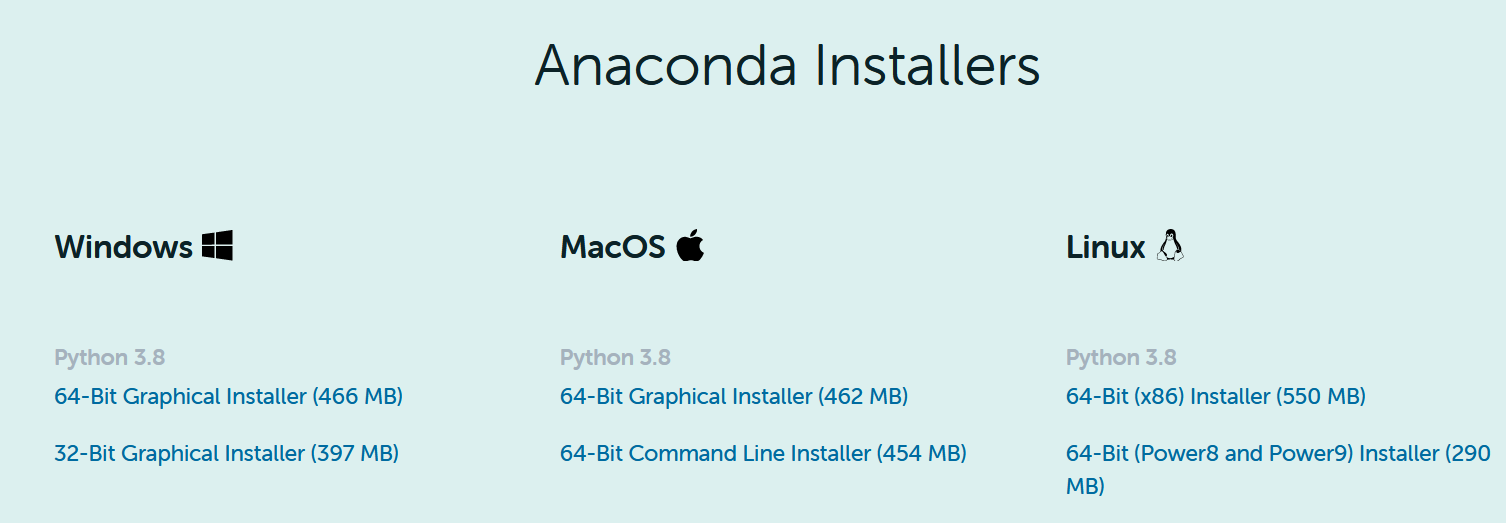
\includegraphics{anaconda}
  \caption{Der Download-Bereich von Anaconda (Ausschnitt).}%
\label{fig:anaconda}
\end{marginfigure}

Falls Sie auf Ihrem Endgerät zwei Accounts, einen Administrator- bzw.\ root-Account und einen Account fürs alltägliche Arbeiten, verwenden, seien Sie bitte vorsichtig.
Die Installation von Anaconda erfordert keine erhöhten Rechte.
Eine Installation mit einem Nutzer mit erhöhten Rechten (z.\,B. \emph{root} oder \emph{admin}) kann u.\,U. dazu führen, dass Anaconda nur für diesen einen Nutzer mit erhöhten Rechten installiert ist bzw.\ dass es zu Problemen mit der Rechteverwaltung kommt.
In der Vergangenheit hat ein erneutes Installieren von Anaconda dieses Problem dann \emph{nicht} beheben können.

Folgen Sie den Installationsschritten und konsultieren Sie im Fehlerfall offizielle Quellen (wie z.\,B. \url{https://docs.anaconda.com/anaconda/install/}) oder Foren.

\newthought{Warum werden Jupyter Notebooks eingesetzt?}
Im Bereich Maschinelles Lernen und Data Science spielen Jupyter Notebooks eine immer größere Rolle%
\cite{perkel_why_2018,hiltch_jupyter_2019}.
Hierbei bezeichnen Jupyter Notebooks gleichzeitig das Medienformat als auch die Standard-IDE.
Das Medienformat ist auf JSON-Basis und enthält u.\,a.\ Text (mit Unterstützung für HMTL), Bilder, ausführbaren Code und den persistierten Outpt ebendieses.
Die gleichnamige IDE kann Jupyter Notebooks öffnen, den enthaltenen Code ausführen, die vom Code erzeugten Visualisierungen nah an diesem platziert anzeigen und das Ergebnis auch wieder speichern.
Die Seminarleitung empfiehlt neuen Benutzern die Verwendung der Standard-IDE Jupyter Notebook für das Bearbeiten der Aufgaben.
Rufen Sie nach dem Download den Installer auf und folgen Sie den Installationsschritten.
Konsultieren Sie im Fehlerfall offizielle Quellen des Herstellers (wie z.\,B. \url{https://docs.anaconda.com/anaconda/install/}) oder Foren (wie z.\,B. \url{https://stackoverflow.com}).


\section{Bezug der Seminar-Materialien}
\label{sec:git-clone}

Klonen Sie das git-Repository
\url{https://github.com/1kastner/machine-learning-hype-or-hybris},
damit Sie die Seminar-Materialien lokal haben -- dies umfasst nur den Programmierteil des Seminars.
Am einfachsten ist es, wenn Sie die Dateien lokal unterhalb des Ordners \texttt{Eigene Dateien} ablegen.
Denn in diesem Ordner öffnet sich standardmäßig JupyterLab.
Falls Sie noch nie mit git gearbeitet haben, lesen Sie bitte die nächsten Absätze.

\newthought{Warum sollte ich git lernen?}
Für die Versionsverwaltung ist git quasi der Standard und wird immer häufiger auch außerhalb der Software-Entwicklung, aus der sie ursprünglich stammt, eingesetzt.
Deswegen lohnt es sich für (fast) jeden, sich Fähigkeiten mit diesem Tool anzueignen.
Das Original-Tool ist ein Kommandozeilentool, welches über \url{https://git-scm.com/} heruntergeladen werden kann.
Wer lieber grafische Oberflächen mag, kann sich eine von vielen GUI Clients%
Das Versionierungssystem \texttt{git} ist ursprünglich als ein Kommandozeilentool entwickelt worden, welches über \url{https://git-scm.com/} heruntergeladen werden kann.
Wer lieber grafische Oberflächen mag, kann sich eine von vielen GUI-Clients%
\sidenote{Eine Liste ist auf \url{https://git-scm.com/download/gui/win} zu finden.}
aussuchen.
Hier sollte neben dem Betriebssystem auch die ggf.\ kostenpflichtige Lizenz beachtet werden.
Einige Lizenzen unterscheiden z.\,B. zwischen der privaten Verwendung und der Verwendung im Arbeitskontext.
Bis zum Start des Workshops werden u.\,U. die Materialien noch überarbeitet oder erweitert.
Aktualisieren Sie also bitte regelmäßig Ihre vorliegende Version über ein \texttt{git pull} bzw.\ durch das Klicken auf den Button \enquote{Pull} im GUI-Client Ihrer Wahl.

\newthought{Ist es für das Seminar zwingend notwendig, git zu lernen?}
Falls Ihnen git unbekannt ist und Sie keine Zeit dafür haben, sich mit git auseinanderzusetzen, gibt es auch die Möglichkeit, den Inhalt als ZIP-Ordner herunterzuladen.
Klicken Sie dafür auf den Button, wie er in Abbildung\,\ref{fig:github} zu sehen ist.
Falls Lernmaterialien später noch angepasst werden, müssen Sie diese dann allerdings erneut herunterladen und in einem neuen Ordner entpacken.

\begin{marginfigure}
  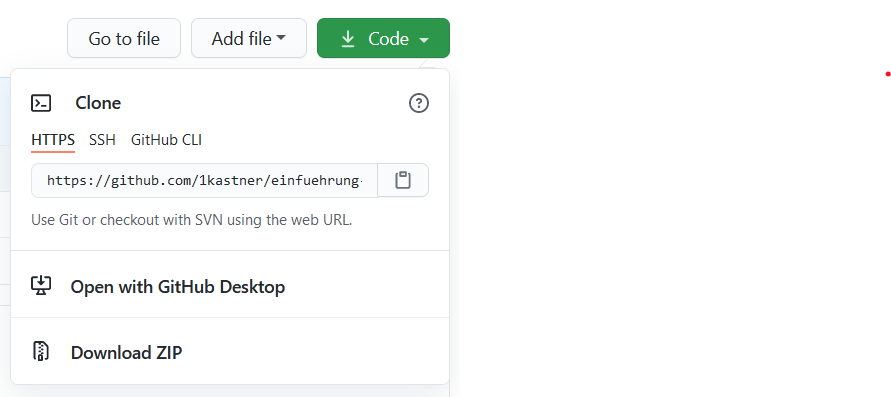
\includegraphics{github-zip}
  \caption{Ein GitHub-Repository bietet verschiedene Möglichkeiten zum Bezug der Inhalte an.}%
\label{fig:github}
\end{marginfigure}


\section{Installation der Bibliotheken}

Mit dem Anaconda Navigator können die im Workshop später benötigten Bibliotheken automatisch installiert werden.
In der Abbildung\,\ref{fig:anaconda-navigator} sehen Sie unten den Button \enquote{Import} (im Screenshot mit einer (1) markiert).
Klicken Sie diesen an.
Damit öffnet sich das Fenster \enquote{Import new environment}.
Klicken Sie hier auf den Ordner in der Zeile, die mit 
\enquote{Specification File}
beginnt (mit einer (2) markiert).
Danach öffnet sich ein Fenster (mit einer (3) markiert), in dem Sie dann zu den heruntergeladenen Dateien navigieren können.
Wählen Sie die \texttt{environment.yml} aus den soeben bezogenen Dateien aus (sie liegt auf der obersten Ebene des Projektordners) und schließen den Vorgang ab.
Das Erstellen der Umgebung nimmt für gewöhnlich einige Zeit in Anspruch.

\begin{figure}[h]
  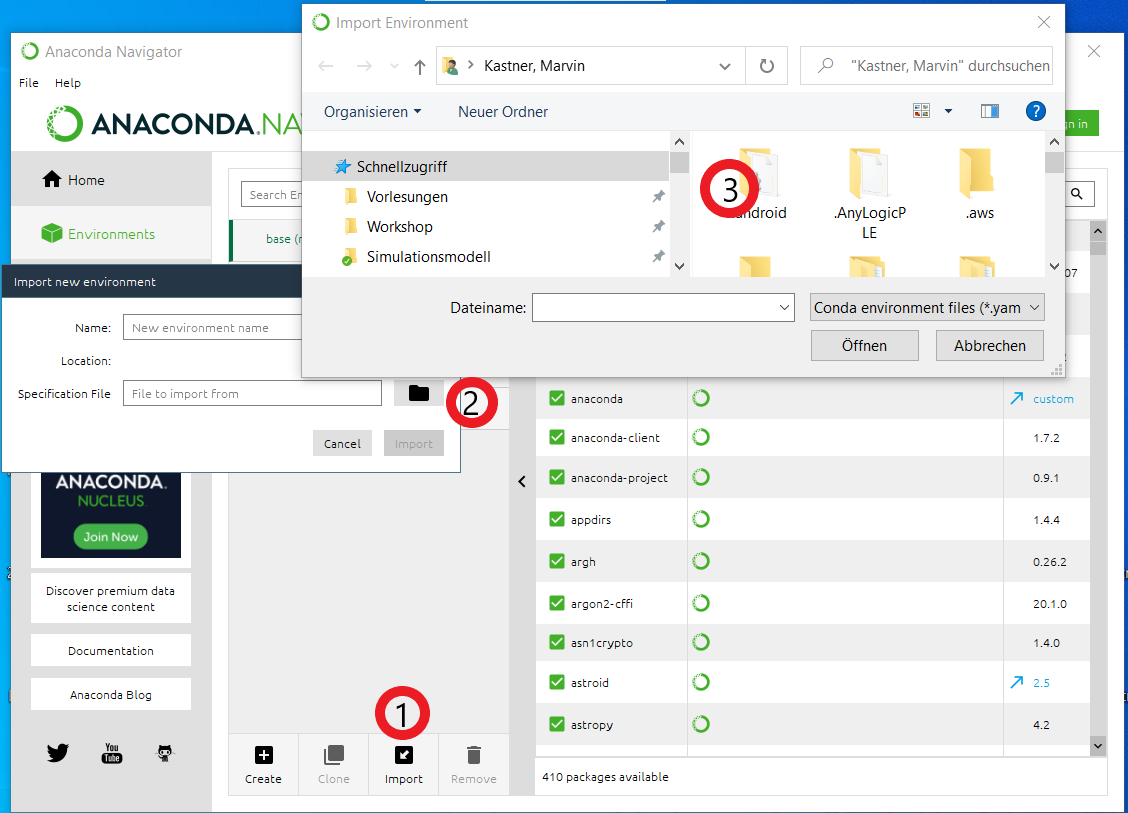
\includegraphics{anaconda-navigator-import-new-environment--mit-reihenfolge}
  \caption{Der Anaconda Navigator erlaubt das Importieren von \texttt{environment.yml}-Dateien.}%
\label{fig:anaconda-navigator}
\end{figure}

\newthought{Warum ist dieser Schritt notwendig?}
Die Jupyter Notebooks, die Sie soeben heruntergeladen haben, benötigen  spezielle Bibliotheken.
Einige werden bereits bei der Installation mit ausgeliefert, andere müssen aber noch nachinstalliert werden.
Auf der obersten Ebene des git-Repositorys befindet sich die Datei \texttt{environment.yml}, in der alle benötigten Bibliotheken aufgelistet werden.
Diese Datei sollten Sie nun bereits auf Ihrem Endgerät in einem lokalen Ordner vorliegen haben.
Die Struktur der Datei \texttt{environment.yml} ist von Anaconda vorgegeben und erlaubt es, die Abhängigkeiten von Bibliotheken automatisch aufzulösen.
Damit man an einem PC in verschiedenen Projekten unterschiedliche Versionen einer gleichen Bibliothek haben kann,
strukturiert Anaconda die zu einem Projekt gehörenden Bibliotheken standardmäßig in Umgebungen (eng. Environments).
Für das Seminar erstellen wir die Umgebung \texttt{intro-jupyter-notebooks} basierend auf der gegebenen \texttt{environment.yml}.

\newthought{Aber ist es denn notwendig, hier mit einer GUI zu arbeiten?}
Natürlich gibt es auch ein Kommandozeilentool, das bereits mit Anaconda ausgeliefert worden ist.
Es heißt \texttt{conda}.
Unter Windows wird dies je nach Auswahl während der Installation nicht in die Pfad-Variable mit aufgenommen.
Dann steht Ihnen immer noch die \emph{Anaconda Prompt} zur Verfügung.
Weitere Informationen gibt es auf
\url{https://docs.anaconda.com/anaconda/install/verify-install/#conda}.
Auf
\url{https://docs.conda.io/projects/conda/en/latest/user-guide/tasks/manage-environments.html#creating-an-environment-from-an-environment-yml-file}
wird erläutert, wie eine existierende \texttt{environment.yml} eingelesen werden kann.
Folgen Sie der Anleitung und erstellen Sie die passende Umgebung.

\section{Start von JupyterLab}

Nun ist JupyterLab einsatzbereit.
Es kann nun über den Anaconda Navigator gestartet werden.
In Abbildung~\ref{fig:start-jupyterlab} ist dies abgebildet.
Zunächst wird links Menü
(im Screenshot mit einer (1) markiert)
\enquote{Home} ausgewählt.
Im zweiten Schritt muss die Umgebung \texttt{intro-jupyter-notebooks} ausgewählt werden
(mit einer (2) markiert).
Danach startet ein Klicken auf \texttt{Launch} JupyterLab im Browser
(mit einer (3) markiert).
Standardmäßig öffnet sich nun der Browser und dort wird der Inhalt vom Ordner \texttt{Eigene Dateien} angezeigt.

\begin{figure}[h]
  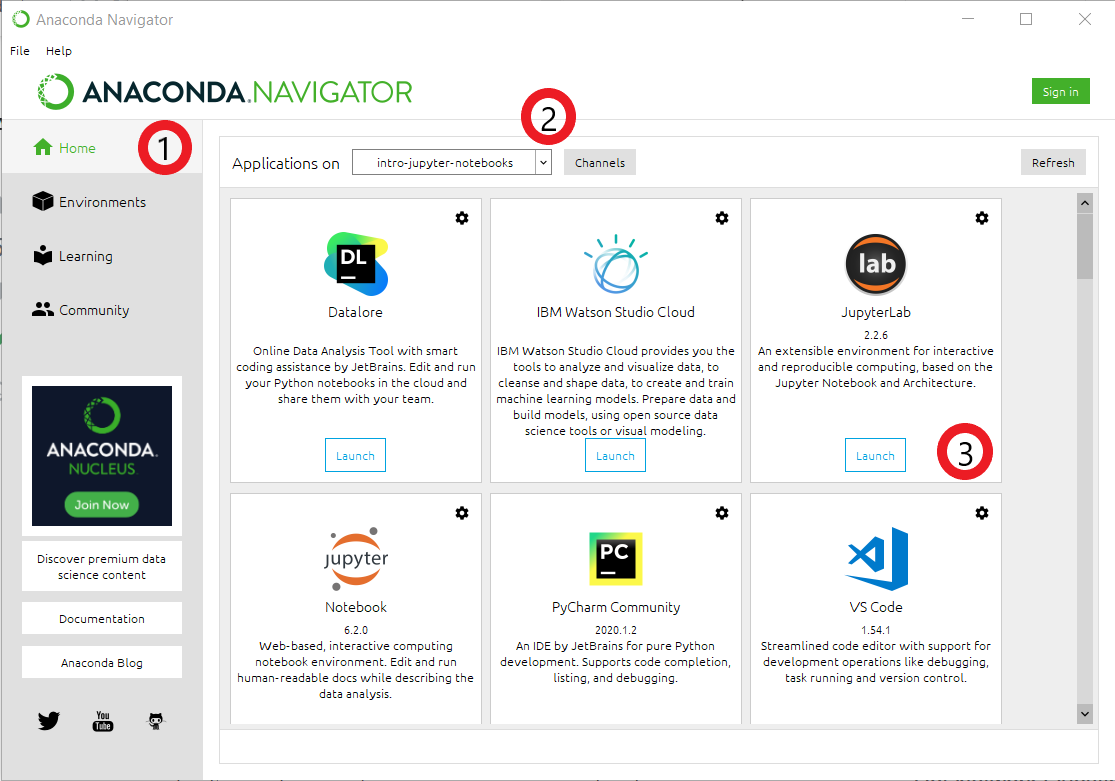
\includegraphics{anaconda-navigator-jupyterlab--mit-reihenfolge}
  \caption{Aus dem Anaconda Navigator kann JupyterLab gleich in der richtigen Umgebung gestartet werden.}%
\label{fig:start-jupyterlab}
\end{figure}

\section{Erste Schritte mit JupyterLab}

Wenn Sie die Workshop-Materialien wie unter Abschnitt \enquote{\nameref{sec:git-clone}} angegeben unterhalb des Ordners \texttt{Eigene Dateien} abgelegt haben, 
können Sie in JupyterLab zum Ordner 
\texttt{00-Installationscheck}
navigieren und dort das Jupyter Notebook (die Datei mit der Endung \texttt{.ipynb}) mit einem Doppelklick öffnen.

 und dort überprüfen, ob Sie alle Zellen ausführen können.
Falls es Fehlermeldungen gibt, melden Sie sich gerne bereits im Vorwege an die Workshop-Leitung.
Falls Sie noch keine Erfahrungen mit Python haben und Sie Interesse haben, sich in diese Sprache einzudenken,
können Sie sich die Einführungsmaterialien unter
\texttt{01-Einfuehrung-in-Python}
anschauen.

\begin{figure}[h]
  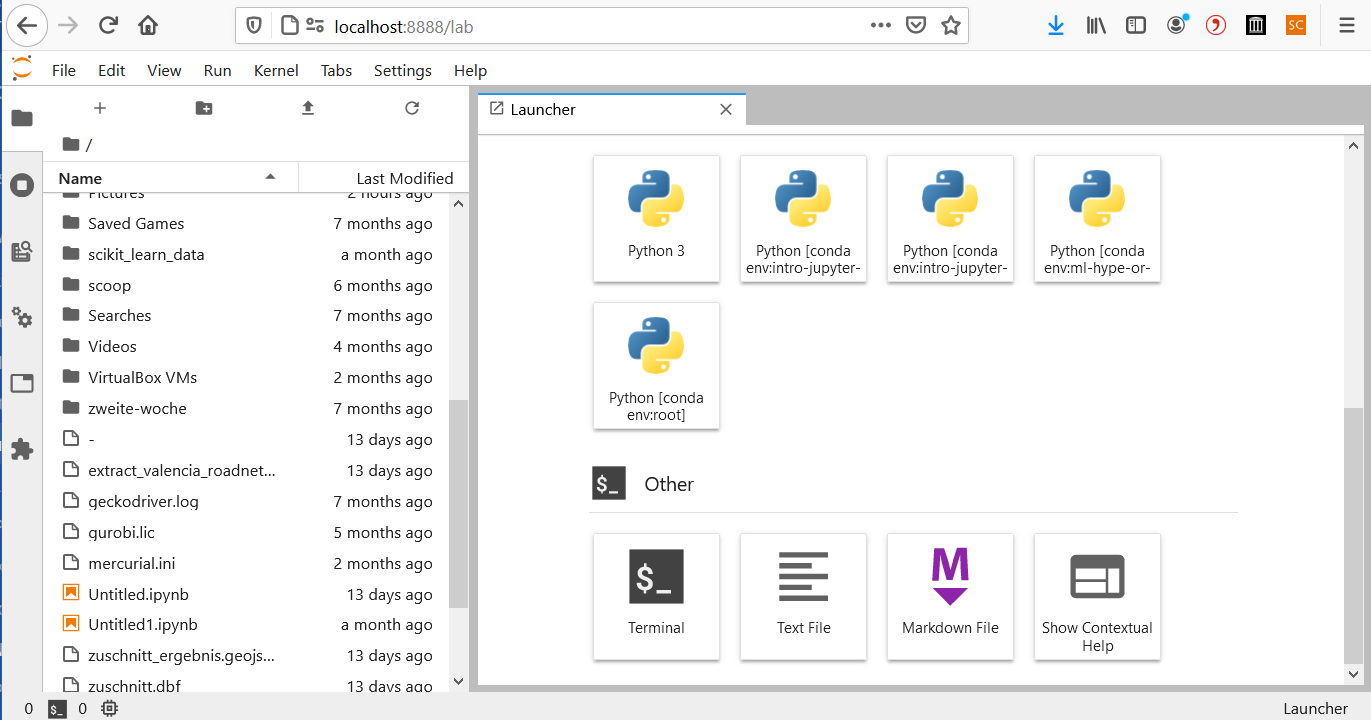
\includegraphics{jupyterlab-running}
  \caption{In JupyterLab können links alle Dateien und Ordner aus dem Ordner \emph{Eigene Dateien} betrachtet werden.}%
\label{fig:start-jupyterlab}
\end{figure}

\bibliography{vorbereitung-auf-das-seminar}
\bibliographystyle{plainnat}

\end{document}
